%! suppress = MultipleIncludes
%! Author = tom.koptel
%! Date = 31/10/2020

% Preamble
\documentclass[a4paper,12pt]{article}

%Ukrainian-specific packages
%--------------------------------------
\usepackage[T2A]{fontenc}
\usepackage[utf8]{inputenc}
\usepackage[ukrainian]{babel}
%--------------------------------------

% Extensions
%--------------------------------------
\usepackage{amssymb,amsfonts,amsmath,cite,enumerate,float,indentfirst}
%--------------------------------------

%Graphics-specific packages
\usepackage{graphicx}
\graphicspath{ {./images/} }

%Code-specific snippets
%--------------------------------------
\usepackage{listings}
\usepackage{xcolor}

\definecolor{codegreen}{rgb}{0,0.6,0}
\definecolor{codegray}{rgb}{0.5,0.5,0.5}
\definecolor{codepurple}{rgb}{0.58,0,0.82}

\lstdefinestyle{light}{
commentstyle=\color{codegreen},
keywordstyle=\color{magenta},
numberstyle=\tiny\color{codegray},
stringstyle=\color{codepurple},
basicstyle=\ttfamily\footnotesize,
breakatwhitespace=false,
breaklines=true,
captionpos=b,
keepspaces=true,
numbers=left,
numbersep=5pt,
showspaces=false,
showstringspaces=false,
showtabs=false,
tabsize=2
}

\lstset{style=light}
%--------------------------------------

%Hyphenation rules
%--------------------------------------
\usepackage{hyphenat}
\hyphenation{ма-те-ма-ти-ка вос-ста-нав-ли-вать}
%--------------------------------------

% Bibliograffy
%--------------------------------------
\usepackage{comment}
\usepackage[backend=biber, style=numeric, sorting=anyt]{biblatex}
\bibliography{theme1}
\bibliographystyle{ieeetr}
%--------------------------------------

% Page geometry
%--------------------------------------
\usepackage{geometry} % Меняем поля страницы
\geometry{left=2cm} % левое поле
\geometry{right=1.5cm} % правое поле
\geometry{top=1cm} % верхнее поле
\geometry{bottom=2cm} % нижнее поле
%--------------------------------------

\title{Представлення зображень у пам’яті комп’ютера.}
\author{Коптель Aртем Олегович}
\date{Листопад 2020}

% Document
\begin{document}

    \begin{titlepage}
    \newpage

    \begin{center}
        УЖГОРОДСЬКИЙ НАЦІОНАЛЬНИЙ УНІВЕРСИТЕТ \\
    \end{center}

    \vspace{8em}

    \begin{center}
        \Large Факультет інформаційних технологій \\
    \end{center}

    \vspace{2em}

    \begin{center}
        \textsc{\textbf{Представлення зображень \linebreak у пам’яті комп’ютера}}
    \end{center}

    \vspace{6em}



    \newbox{\lbox}
    \savebox{\lbox}{\hbox{Василь Олександрович Лавер}}
    \newlength{\maxl}
    \setlength{\maxl}{\wd\lbox}
    \hfill\parbox{11cm}{
    \hspace*{5cm}\hspace*{-5cm}Студент:\hfill\hbox to\maxl{Коптель Артем Олегович\hfill}\\
    \hspace*{5cm}\hspace*{-5cm}Викладач:\hfill\hbox to\maxl{Василь Олександрович Лавер}\\
    \\
    \hspace*{5cm}\hspace*{-5cm}Група:\hfill\hbox to\maxl{Комп’ютерні науки та інформаційні технології}\\
    }


    \vspace{\fill}

    \begin{center}
        Ужгород \\2020
    \end{center}

\end{titlepage}

    \newpage

    \tableofcontents
    \newpage


    \section{Вступ}\label{sec:intr}
    Зображення - найкращий спосіб опису дійсності.
    Людина на багато краще розпізнає зображення ніж тескст або аудіозапис.
    В цьому немає нічого дивного, адже зір та розпізнавання образів є критичним з точки зору виживання.
    Томy і не дивно, що основний спосіб взаємодії з комп'ютером, це робота з засобами виводу такми як монітор.

    Зображення, визначене з математичної точки зору, вважається функцією двох реальних змінних, наприклад, a(x, y) де "а" - амплітуда (наприклад, яскравість) зображення з координатою (x, у).
    Крім того, можна вважати, що зображення містить підзображення, які іноді називають регіонами інтересів, ROI або просто регіонами.
    Ця концепція відображає той факт, що зображення часто містять колекції предметів, кожен з яких може бути основою для регіону.

    В даній роботі ми розглянемо теорертичний матеріал, щоби відповісти на питання: "Яким чином реалізоване представлення зображення у пам'яті комп'ютера".
    Спочатку ми розглянемо загальні відомості.
    Далі опишемо поняття піксель, воксель, растрове та векторне зображення.
    Обговоримо поняття каналів і опишемо обєми даних використаних для опису зображення.


    \section{Репрезентація пікселя}\label{sec:pixel_definition}
    Зображення можно описати концепцією 3-D обєму (I), який можна описати математично:
    \[ \alpha = I \rightarrow R, I \subset R \]
    Таким чином, кожний піксель зображення має дійсне число, яке його репрезинтує.
    Однак, в реальності зручніше зберігати та ефективніше опрацьовувати цілі числа замість чисел з плаваючою точкою.
    Тобто, значення пікселів описані цілими числами.

    \subsection{Глибина біту (Bit Depth)}\label{subsec:bit_depth}
    Діапазон значень, який використовується для опису довільного формату зображення визначається глибиною біта.
    Діапазон можна описати, як відрізок \([0, 2^{bitdepth - 1}]\).
    Наприклад, 8-бітне зображення буде мати діапазон \([0, 2^{8} - 1] = [0, 255]\).
    Таким чином, чим вище значення глибину біту тим більше потрібно дискового простору та пам'яті, щоби опрацювати зображення.
    Більшість поширених фото-форматів, таких як jpeg, png тощо, використовують 8-біт для зберігання і набувають лише позитивні значення.

    Якщо потрібна більш висока точність (наприклад, наукове застосування), тоді використовують глибину біту вищих значень.
    Наприклад, 16-bit зображення буде мати значення пікселів в діапазоні [0, 65535], де  \(65535 = 2^{16}\).
    Для зображень, що мають як позитивні, так і негативні значення пікселів, діапазон становить [−32768, + 32768].
    Загальна кількість значень у цьому випадку становить \(65536(=2^{16})\) або бітова глибина 16.
    Прикладом такого зображення є зображення CT DICOM.

    Коли потрібно зробити зображення з вискоким рівнем точності тоді використовують більшу глубину біта.
    Наприклад, значення пікселя від 1000 описує колір кістки.
    При використанні 8-бітного діапазону використовується значення 255, тобто білий.
    Всі значення більші за 255 будуть інтерпольовані, як білий колір, в свою чергу ми втрачаємо точність.

    \subsection{Формат та глибина. Відношення}\label{subsec:formats}
    \begin{itemize}
        \item DICOM - 1 канали по 16-bit, отже глибина 16-біт.
        \item RGB - 3 канали по 8-bit, отже глибина 24-біта.
        \item TIFF - 5 каналів по 16-bit, отже глибина 80-біта.
    \end{itemize}


    \section{Піксель та Воксель. Загальні відомості}\label{sec:pixel_voxel}
    Кожен піксель має певні розміри (XY, де переважно X = Y) і певне значення відтінку сірого, щоби описати матеріал, який він представляє.
    Зображення розташовані на певній відстані (Z).
    Ця відстань надає пікселям певної глибини.
    VOlume piXEL називається вокселем, він має розміри XYZ.
    Тобто додаючи третій параметр до значення ми розширюємо поняття.

    Для того щоби краще зрозуміти воксель, переглянемо інформацію про піксель.

    Піксель на рисунку 1. можна сприймати як контейнр, який збирає світло або електрони, залежно від типу використовуваного детектора.
    Один піксель на зображенні охоплює якусь відстань у фізичному світі.
    Наприклад, на рисунок 1. стрілки вказують ширину та висоту пікселя, розміщеного поруч із трьома іншими пікселями.
    У цьому випадку ширина та висота цього пікселя становлять 0,5 мм.

    \begin{figure}
        \label{fig:image1}
        \centering
        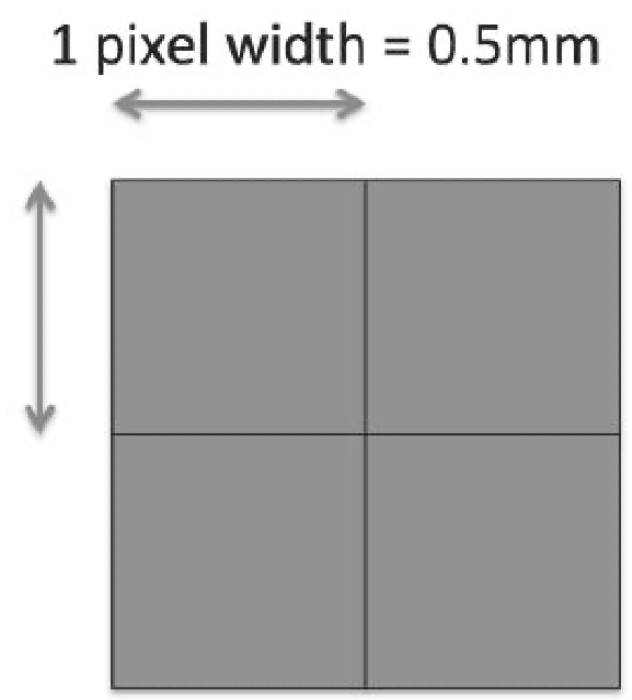
\includegraphics[scale=0.5]{image1.png}

        Рис. 1. Фізичне відображення пікселя.
    \end{figure}

    Таким чином, у фізичному просторі подолання відстані 0,5 мм еквівалентно подоланню 1 пікселя в піксельному просторі.
    З усіх практичних цілей можна припустити, що детектори мають квадратні пікселі, тобто ширина та висота пікселів однакові.

    Розмір пікселів може бути різним для різних методів зображення та різних детекторів.
    Наприклад, розмір пікселів більший для CT порівняно з mikro-CT.

    \subsection{Воксель в медицинi.}\label{subsec:voxel_med}
    У медичній та мікроскопічній зйомках частіше отримують тривимірні зображення.
    У таких випадках розмір пікселя матиме третій вимір, а саме глибина пікселів.
    Термін піксель, як правило, застосовується до 2D і замінюється вокселем у 3D-зображеннях.

    Більшість поширених форматів зображень, таких як DICOM, nifti та деякі формати зображень з мікроскопом, містять розмір вокселів у своєму заголовку.
    Отже, коли такі зображення читаються у програмі візуалізації або обробки зображень, може бути здійснений точний аналіз та візуалізація.
    Але якщо зображення не містить інформації в заголовку або якщо програма візуалізації чи обробки зображень не може правильно прочитати заголовок, важливо використовувати правильний розмір вокселя для аналізу.


    \section{Система координат}\label{sec:coordinate_system}
    Нам потрібна система координат для опису зображення.
    Cистема координат, що використовується для розміщення елементів по відношенню один до одного, називається користувацьким простором, оскільки це координати, які користувач використовує для визначення елементів і розташування їх по відношенню один до одного.
    Система координат, використана для відображення графіки (наприклад механізм рендерінгу для Android та iOS платформ), має початок у верхньому лівому куті, вісь x простягається праворуч, а вісь y - вниз.

    \begin{figure}
        \label{fig:image2}
        \centering
        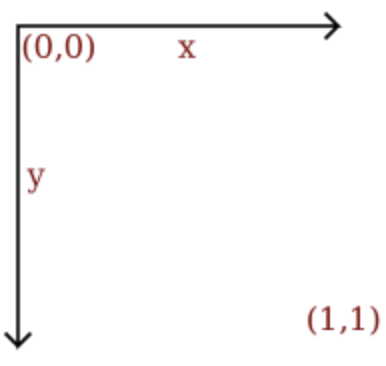
\includegraphics[scale=0.5]{image2.png}

        Рис. 2. Система координат.
    \end{figure}

    \pagebreak


    \section{Векторні зображення.}\label{sec:vector_images}
    Одним із способів описати зображення за допомогою тексту є оголошення його вмісту за допомогою положення та розміру геометричних форм і фігур, таких як лінії, криві, прямокутники та кола;такі зображення називаються \textbf{векторними}.

    \begin{figure}
        \label{fig:image3}
        \centering
        
\includegraphics[scale=0.5]{image3.png}

        Рис. 3. Векторне зображення обличчя.
    \end{figure}

    \begin{lstlisting}[style=light, language=Python,label={lst:vectorimg},caption=Приклад векторного зображення]
            draw circle
                 center        0.5, 0.5
                 radius        0.4
                 fill-color    yellow
                 stroke-color  black
                 stroke-width  0.05
            draw circle
                 center        0.35, 0.4
                 radius        0.05
                 fill-color    black
            draw circle
                 center        0.65, 0.4
                 radius        0.05
                 fill-color    black
            draw line
                 start         0.3, 0.6
                 end           0.7, 0.6
                 stroke-color  black
                 stroke-width  0.1
    \end{lstlisting}

    \subsection{Визначаємо форму}\label{subsec:defining_shapes}

    Попередній опис зображення можна розглядати як "рецепт приготування", як намалювати зображення.
    Він містить геометричні примітиви, такі як лінії, криві та кола, що описують колір, а також відносний розмір, положення та форму елементів.
    Коли підготовка зображення до відображення повинна бути перетворена у \textbf{растрове зображення}, цей процес називається \textbf{растеризацією}.

    Векторне зображення не залежить від роздільної здатності, це означає, що ви можете збільшити або зменшити зображення, не впливаючи на якість виводу.
    Векторне зображення не втрачає якість при масштабувані оскільки ми працюємо з декларативним синтаксисом, тобто інструкцією.
    Таким чином ми можемо змінювати розмір полотна і не втрачати в якості, оскільки зображення буде пераховане в межах полотна.
    Векторні зображення є найкращим способом представлення шрифтів, логотипів та багатьох ілюстрацій.


    \section{Растрові зображення}\label{sec:bitmap_image}

    Растрові, зображення є «цифровими фотографіями», вони є найпоширенішою формою для представлення природних зображень та інших видів графіки, які багаті на деталі.
    Растрові зображення - це те, як графіка зберігається у відеопам’яті комп’ютера.
    Термін растрове зображення стосується того, як заданий шаблон бітів у пікселі відображається до певного кольору.
    Попередній опис зображення можна розглядати як "рецепт приготування", як намалювати зображення, він містить геометричні примітиви, такі як лінії, криві та кола, що описують колір, а також відносний розмір, положення та форму елементів.
    Коли підготовка зображення до відображення повинна бути перетворена у растрове зображення, цей процес називається растеризацією.

    Растрові зображення набувають форми масиву, де значення кожного елемента, який називається елементом \textbf{піксельного(pixel) зображення}, відповідає кольору цієї частини зображення.
    Де горизонтальна лінія на зображенні називається \textbf{лінією сканування(scan line)}.

    Буква "а" може бути представлена в матриці 12x14, як показано на малюнку 3., значення в матриці відображають яскравість \textbf{пікселів} (елементів зображення).
    Більші значення відповідають світлішим областям, тоді як нижчі значення темнішим.

    \begin{figure}
        \label{fig:image4}
        \centering
        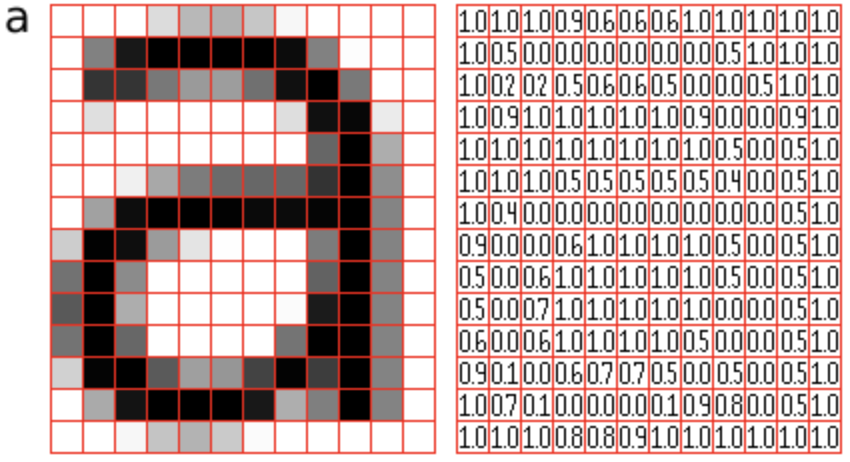
\includegraphics[scale=0.5]{image4.png}

        Рис. 4. Растеризована форма букви "а" збільшена в 16 разів за допомогою подвоєння пікселів
    \end{figure}

    \subsection{Растровий розмір}\label{subsec:raster_sdimensions}
    Кількість горизонтальних і вертикальних зразків у піксельній сітці називається \textbf{растровим розміром(raster dimension)}, вона визначається як ширина X висота.


    \section{Дискретизація або вибірка (Sampling)}\label{sec:sampling}
    "Вибірка - це процес перетворення сигналу (наприклад, функції безперервного часу або простору) в числову послідовність (функція дискретного часу або простору).
    Процес також називається аналого-цифровим перетворенням або просто оцифровкою"~\cite{wiki_sampling:2}.

    Вимірюючи значення для пікселя, приймається середній колір області навколо місця розташування пікселя.
    Спрощеною моделлю є вибірка квадрата, це називається \textbf{коробчатим фільтром}, більш фізично точне вимірювання полягає в обчисленні зваженого середнього за Гаусом значення.
    Більше значення ваги набувається на координатах визначення пікселя, а менші значення ваги в областях навколо пікселів~\cite{gimp:1}.

    При сприйнятті растрового зображення людське око "змішує" значення пікселів між собою, відтворюючи ілюзію безперервного зображення, яке воно представляє.
    Іншими словами, око сприймає форму як різницю переходу між більшим та меньшим значення ваги пікселя (різниця між відтінками).

    \subsection{Приклад дискретизації}\label{subsec:example_of_sampling}
    Зображення 256 х 256 пікселів, яке охоплює фізичну площу 100 х 100 мкм, має щільність вибірки 256/100 = 2,56 зразка на мікрон як вздовж X, так і Y.
    Еквівалентно, розмір вибірки вздовж будь-якого з цих напрямків становить 100/256 ~ 0,391 мкм = 391 нм.
    Чи достатньо цього для сучасних умов, визначається ідеальною частотою дискретизації~\cite{svi_sampling:3}.

    Зміна коефіцієнта масштабування скануючого мікроскопа для сканування меншої фізичної площі, скажімо, 70 х 70 мкм, зберігаючи однакову кількість пікселів у записаному зображенні, 256 х 256 пікселів, дозволяє отримати роздільну здатність, зменшуючи розмір вибірки: 70 / 256 ~ 0,273 мкм = 273 нм.
    Ми отримуємо більше зразків на певній фізичній відстані, дозволяючи розрізнити більше деталей.
    Однак це обмежується дифракцією на лінзах, а вибірка, що перевищує ідеальну швидкість, не покращує ситуацію~\cite{svi_sampling:3}.

    Мікроскопічному масштабуванню можна протиставити "цифрове збільшення": обрізання та інтерполяція отриманих даних.
    Цифрове (після придбання) масштабування не забезпечує більше фізичної інформації або кращої роздільної здатності, структури не вирішуються краще.
    Він споживає ресурси зберігання та пам'яті.
    Дві різні функції, які виглядають як накладені через обмеження роздільної здатності, перекриуть одна іншу після цифрового масштабування~\cite{svi_sampling:3}.


    \section{Роздільна здатність}\label{sec:resolution}
    \textbf{Роздільна здатність} - це вимірювання щільності дискретизації, роздільна здатність растрових зображень дає зв'язок між розмірами пікселів та фізичними розмірами.
    Найбільш часто використовується вимірювання - ppi(pixel per inch), пікселів на дюйм.

    Різниця між \textbf{ppi} та \textbf{dpi} - це різниця між пікселями та точками - пікселі можуть представляти кілька значень, тоді як крапка - це монохромне пляма чорнила або тонера одного барвника, виготовленого принтером.
    Принтери використовують процес, який називається \textbf{напівтонування}, для створення монохромного малюнка, що імітує діапазон рівнів інтенсивності.

    \subsection{Мега піксель}\label{subsec:megapixels}
    Мегапікселі відносяться до загальної кількості пікселів у захопленому зображенні, простішою метрикою є \textbf{растрові розміри}, які представляють кількість горизонтальних та вертикальних зразків у сітці вибірки.
    Зображення зі співвідношенням сторін 4:3 із розміром 2048x1536 пікселів містить загалом 2048x1535 = 3145728 пікселів;
    приблизно 3 мільйони, таким чином, це 3-мегапіксельне зображення~\cite{gimp:1}.

    \begin{figure}
        \label{fig:image5}
        \centering
        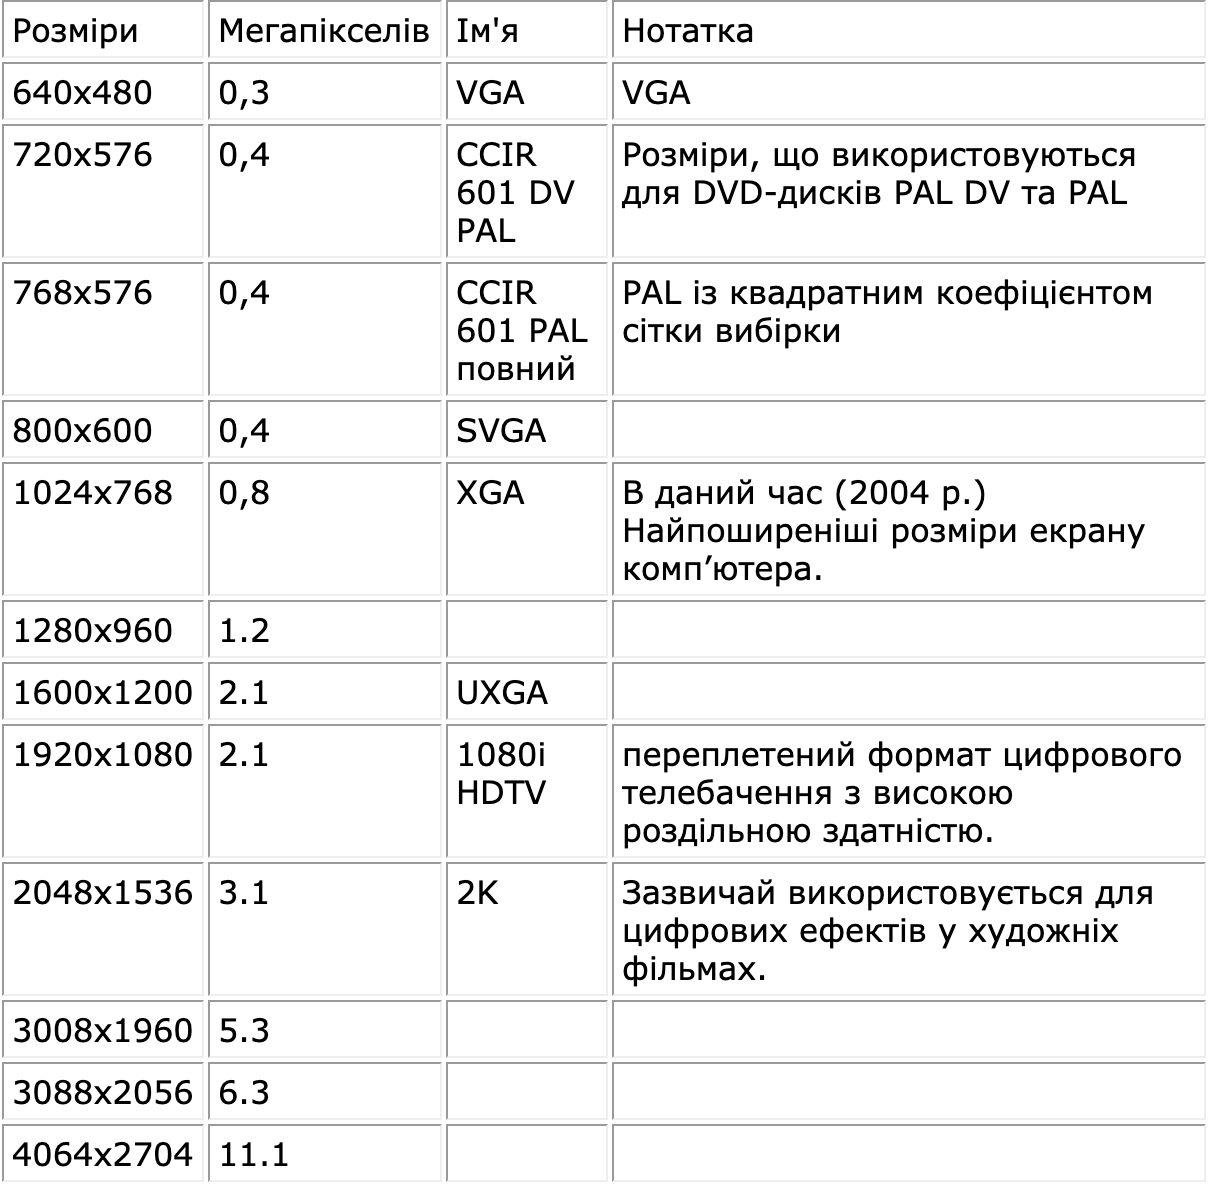
\includegraphics[scale=0.5]{image5.png}

        Рис. 5. Загальні растрові розміри
    \end{figure}

    \subsection{Масштабування / Передискретизація (Scaling / Resampling)}\label{subsec:scaling_resampling}
    Коли нам потрібно створити зображення з різними розмірами, ніж ми маємо, ми масштабуємо зображення.
    Інша назва масштабування - передискретизація, коли алгоритми передискретизації намагаються відновити вихідне безперервне зображення та створити нову сітку зразків~\cite{gimp:1}.

    \subsection{Зменшення масштабу зображення}\label{subsec:downscaling}
    Процес зменшення растрових розмірів називається децимацією (decimation), це може бути зроблено шляхом усереднення значень вихідних пікселів, що вносять вклад в кожен вихідний піксель~\cite{gimp:1}.

    \subsection{Масштабування зображення вгору}\label{subsec:upscaling}
    Коли ми збільшуємо розмір зображення, ми фактично хочемо створити точки вибірки між вихідними точками вибірки у вихідному растрі, це робиться шляхом інтерполяції значень у сітці вибірки, ефективно вгадуючи значення невідомих пікселів.
    При використанні цифрового масштабування камери камера використовує \textbf{інтерполяцію}, щоб вгадати значення, яких немає на зображенні.


    \section{Глибина зразка (Sample depth)}\label{sec:sample_depth}
    Значення пікселів потрібно зберігати в пам’яті комп’ютерів, це означає, що врешті-решт дані повинні в кінцевому підсумку потрапити у двійкове представлення, просторова безперервність зображення апроксимується інтервалом вибірки в сітці зразків.

    Значення, які ми можемо представити для кожного пікселя, визначаються обраним зразком формату.

    \begin{figure}
        \label{fig:image6}
        \centering
        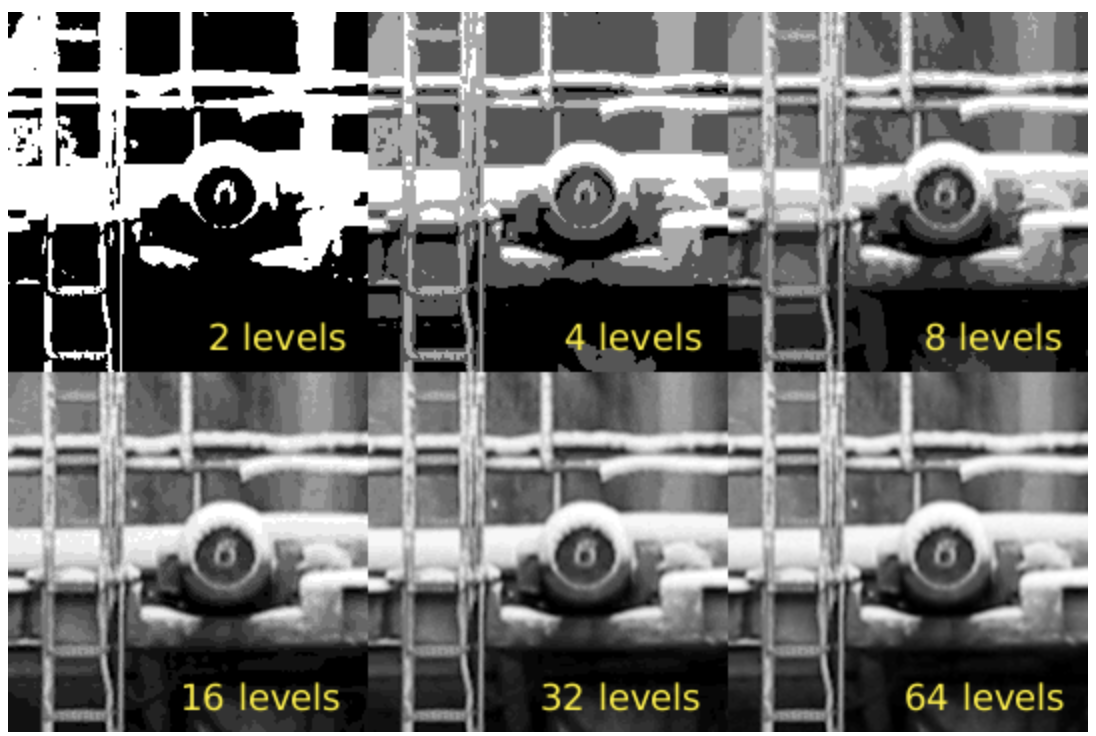
\includegraphics[scale=0.5]{image6.png}

        Рис. 6. Глибина зразка
    \end{figure}

    На рисунку 6 однакова ширина зображеннь.
    Змінюється тільки глибина зразка.
    Зауважте, що області з високою частотою (деталізовані області) мають добрий вигляд, ніж області з низькою частотою.

    \subsection{8 біт}\label{subsec:bit_eight}
    Типовим форматом вибірки є 8-бітові цілі числа, 8-бітові цілі числа можуть представляти лише 256 дискретних значень (\(2^{8} = 256\)), таким чином рівні яскравості квантуються на ці рівні.

    \subsection{12 біт}\label{subsec:bit_twelve}
    Для зображень із високим динамічним діапазоном (зображення з деталізацією як у тіні, так і у світлих місцях) 8-бітне 256 дискретних значень не забезпечує достатньої точності для збереження точного зображення.
    Деякі цифрові камери внутрішньо працюють з більш ніж 8-бітними зразками, камери вищого класу також надають RAW-зображення, які часто мають 12 біт (\(2^{12} = 4096\)).

    \subsection{16 біт}\label{subsec:bit_sixteen}
    Формати зображень PNG і TIF підтримують 16-бітні зразки, багато програм обробки зображень та маніпуляцій виконують свої операції в 16-бітному режимі, працюючи над 8-бітними зображеннями, щоб уникнути втрати якості при обробці.

    \subsection{Плаваюча крапка (Floating point)}\label{subsec:floating_point}
    Деякі формати зображень, що використовуються в дослідженнях та у кіноіндустрії, зберігають значення з плаваючою комою.
    Як "звичайні" 32-бітові значення з плаваючою комою, так і спеціальний формат, що називається \textbf{половина(half)}, який використовує 16 біт / зразок.
    Зображення з плаваючою комою корисний як робочий формат, оскільки квантування та обчислювальні помилки зводяться до мінімуму до остаточного відтворення.

    Представлення з плаваючою точкою часто включає HDR, \textbf{високий динамічний діапазон}.
    Зображення з високим динамічним діапазоном - це зображення, що включають значення вибірки, які біліші від білого (вищі значення, ніж 255 для звичайного 8-бітного зображення).
    HDR дозволяє представляти світло сцени з більшим ступенем точності, ніж зображення LDR із \textbf{низьким динамічним діапазоном}.


    \section{Кольори}\label{sec:color}
    Найпоширенішим способом моделювання кольорів в комп'ютерній графіці є кольорова модель RGB, що відповідає способу відтворення кольору як на CRT-моніторах, так і на LCD-екранах / проекторах.

    Кожен піксель представлений трьома значеннями - червоного, зеленого та синього каналів.

    Таким чином, кольорове зображення у форматі RGB використовуватиме втричі більше пам'яті, ніж сіро-кольорове зображення з однаковими розмірами пікселів.

    На рисунку 7 кольорове зображення, складене смугами червоного, зеленого та синього кольорів (це зображення ілюструє побудову дисплея ноутбука, зверніть увагу, що це зображення бажано переглядати на екрані комп'ютера, а не друкувати).

    Одним з найпоширеніших форматів пікселів є 8 біт rgb, де значення червоного, зеленого та синього зберігаються з чергуванням у пам'яті.
    Таке розташування пам'яті часто називають \textbf{кремезним(chunky)}, зберігання компонентів в окремих буферах називається \textbf{площинним(planar)}, і не так часто застосовується.

    \begin{figure}
        \label{fig:image7}
        \centering
        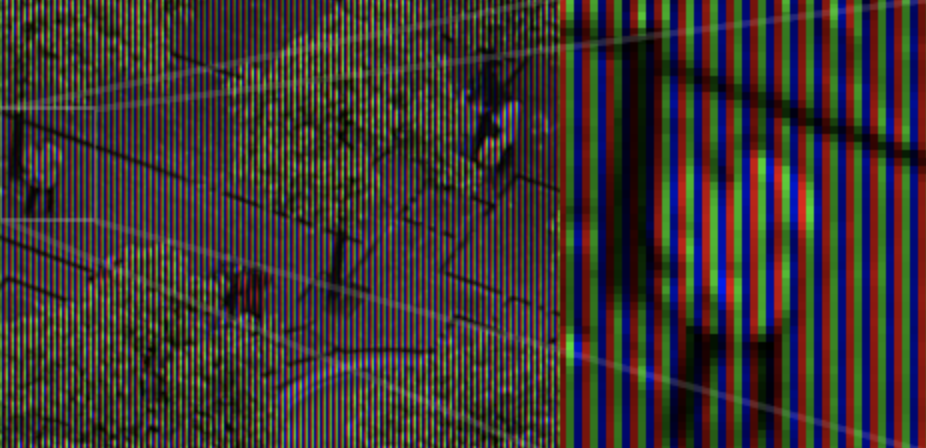
\includegraphics[scale=0.5]{image7.png}

        Рис. 7. Глибина зразка
    \end{figure}


    \section{Палітра / Індексовані зображення}\label{sec:palette}
    Раніше було звичайним зберігати зображення в палетизованому режимі.
    Ми зберігаємо лише номер запису палітри, що використовується для кожного пікселя.
    І для кожного запису палітри ми зберігаємо кількість червоного, зеленого та синього світла.

    На рисунку 8 зліва зображення використовує лише 16 кольорів, праворуч палітра, що використовується для цього зображення.
    Принцип роботи індексованого / палітруваного зображення подібний до того, як працює фарба за номерами.

    \begin{figure}
        \label{fig:image8}
        \centering
        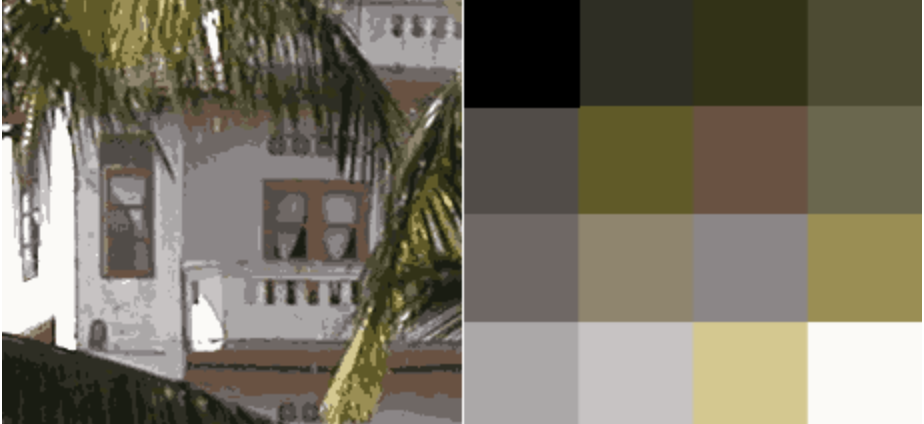
\includegraphics[scale=0.5]{image8.png}

        Рис. 8. Глибина зразка
    \end{figure}


    \section{Стиснення зображення.}\label{sec:image_compression}
    Растрові зображення займають багато пам'яті, \textbf{стиснення зображення} зменшує обсяг пам'яті, необхідної для зберігання зображення.
    Наприклад, 2,1-мегапіксельне 8-бітне RGB-зображення (1600x1200) займає 1600x1200x3 байт = 5760000 байт = 5,5 мегабайт, це нестиснутий розмір зображення.

    \textbf{Коефіцієнт стиснення} - це співвідношення між стисненим зображенням і нестисненим зображенням, якщо згаданий вище приклад зображення зберігався як файл jpeg у розмірі 512 кб, коефіцієнт стиснення становив би 0,5 мб: 5,5 мб = 1:11.


    \section{Стиснення зображення без втрат}\label{sec:lossless_image_compression}
    Коли зображення стискається без втрат, повторення та передбачуваність використовуються для подання всієї інформації, використовуючи менше пам'яті.
    Вихідне зображення можна відновити.
    Одним з найпростіших методів стиснення зображень без втрат є кодування довжини циклу.
    Кодування довжини циклу кодує послідовні та подібні значення, як один маркер у потоці даних.

    На рисунку 9, “Кодування довжини циклу ”, чорно-біле зображення будинку було стиснене кодуванням довжини циклу, растрове зображення розглядається як один довгий рядок чорних / або білих пікселів, кодування - скільки байтів одного кольори виникають один за одним.
    Ми ще більше зменшимо кількість байтів, зайнятих цими 72 числовими значеннями, маючи максимальну довжину інтервалу 15 і кодуючи довші інтервали за допомогою кількох інтервалів, розділених нульовими інтервалами іншого кольору.
    \begin{figure}
        \label{fig:image9}
        \centering
        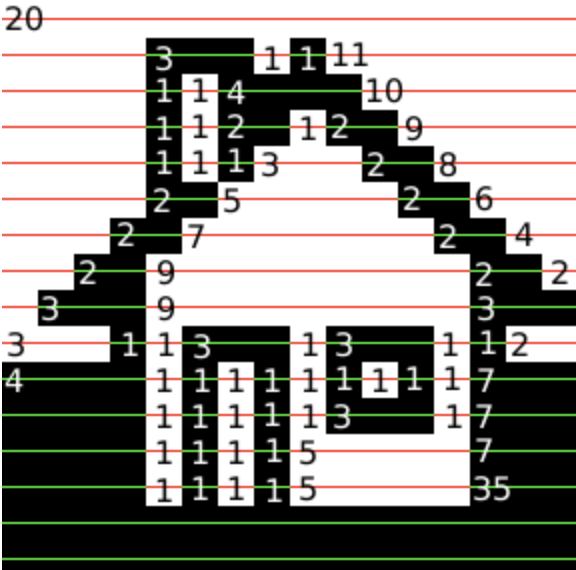
\includegraphics[scale=0.5]{image9.png}

        Рис. 9. Кодування довжини циклу (Run-length encoding)
    \end{figure}

    \begin{lstlisting}[style=light, language=Python,label={lst:vectorimg},caption=Кодування довжини циклу]
        70, 15, 0, 15, 0, 15, 0, 10,
         5, 25, 5, 15, 0, 10,
         5, 27, 6, 15, 0, 12,
         4, 26, 4, 15, 0, 11,
         4, 25, 4, 15, 0, 10,
         6, 24, 6, 15, 0, 9,
         6, 23, 6, 15, 0, 8,
         3, 2, 3, 22, 3, 2, 3, 15, 0, 7,
         3, 2, 3, 21, 3, 2, 3, 15, 0, 6,
         3, 5, 2, 20, 3, 5, 2, 15, 0, 5,
         3, 5, 2, 19, 3, 5, 2, 15, 0, 4,
         3, 7, 2, 18, 3, 7, 2, 15, 0, 3,
         3, 7, 2, 17, 3, 7, 2, 15, 0, 2
        14, 16, 14, 15, 0, 1
         3, 11, 2, 14, 3, 11, 2, 14,
         3, 11, 2, 13, 3, 11, 2, 13,
         3, 13, 2, 12, 3, 13, 2, 12,
         3, 13, 2, 11, 3, 13, 2, 11,
         3, 15, 2, 10, 3, 15, 2, 10,
         3, 15, 2, 8, 3, 15, 2, 8,
         6, 12, 6, 6, 6, 12, 6, 6,
         6, 12, 6, 64 6, 12, 6, 15, 0, 15, 0, 15, 0, 15, 0, 4
    \end{lstlisting}


    \section{Стиснення зображення з втратами}\label{sec:lossy_image_compression}
    Стиснення з втратами використовує здатність людських очей приховувати недосконалість і той факт, що деякі типи інформації важливіші за інші.
    Наприклад, зміни освітленості спостерігаються людиною як більш значущі, ніж зміна відтінку.

    JPEG - це формат файлу, що реалізує стиснення на основі дискретного косинусного перетворення DCT, разом з алгоритмами без втрат, що забезпечує хороші коефіцієнти стиснення.
    Спосіб роботи JPEG найкраще підходить для зображень із безперервними тональними діапазонами, таких як фотографії, логотипи, відсканований текст та інші зображення з безліччю чітких контурів / ліній, отримують більше артефактів стиснення, ніж фотографії.

    \subsection{Втрати через покоління}\label{sec:loss_through_generations}
    Алгоритми стиснення втрат не слід використовувати як робочий формат, лише кінцеві копії слід зберігати у форматі jpeg, оскільки втрати накопичуються протягом поколінь.

    Зображення 10, спеціально побудоване для показу недоліків алгоритму стиснення JPEG, збережене, повторно відкрите та збережене знову 9 разів.

    JPEG найбільш підходить для фотографічного вмісту, коли несприятливий ефект алгоритму стиснення не так очевидний.

    JPEG не підходить як проміжний формат, використовуйте JPEG лише для остаточного розповсюдження, де розмір файлу насправді має значення.

    \begin{figure}
        \label{fig:image10}
        \centering
        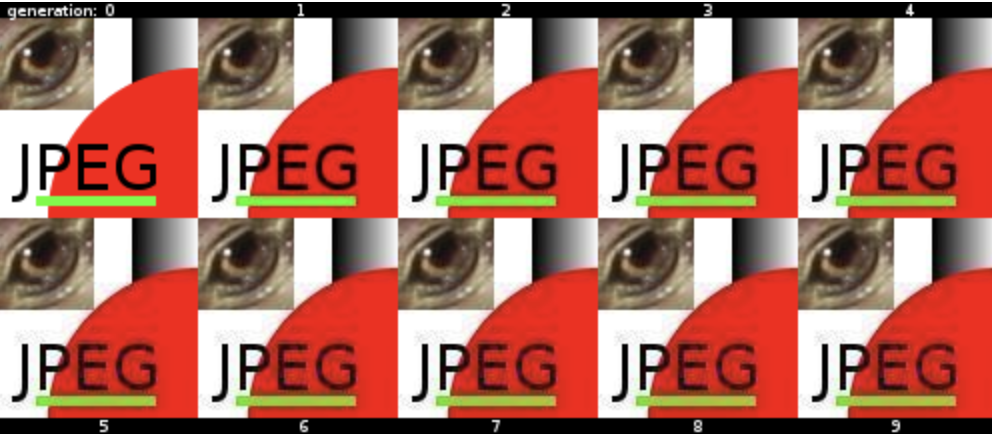
\includegraphics[scale=0.5]{image10.png}

        Рис. 10. Втрата якості через кілька генерацій JPEG
    \end{figure}


    \section{Формати файлів та програми}\label{sec:image_formats}
    Багато програм мають власний внутрішній формат файлу, тоді як інші формати більше підходять для обміну даними.
    У таблицях на малюнках 10 та 11 перелічено деякі поширені формати зображень.

    \begin{figure}
        \label{fig:image11}
        \centering
        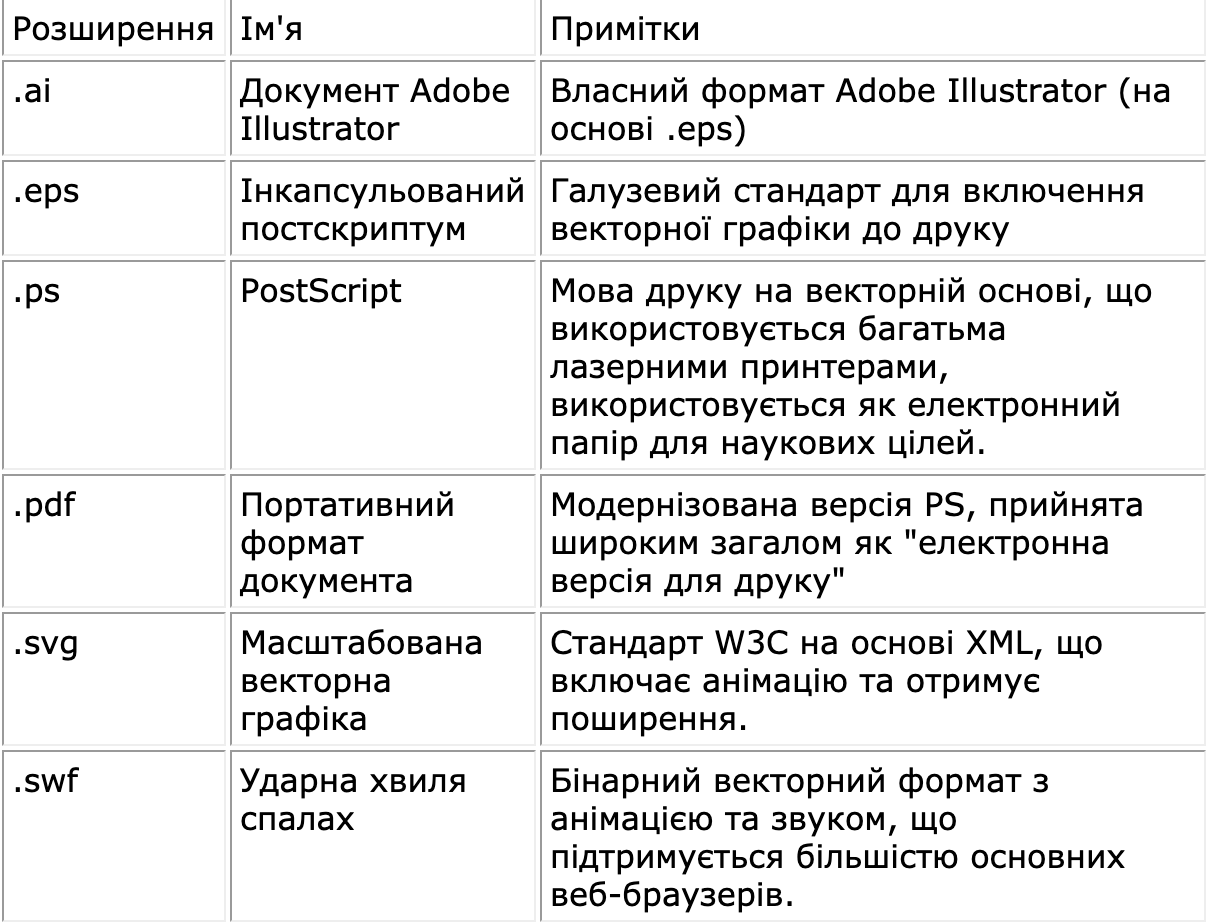
\includegraphics[scale=0.5]{image11.png}

        Рис. 11. Формати векторних файлів.
    \end{figure}

    \begin{figure}
        \label{fig:image12}
        \centering
        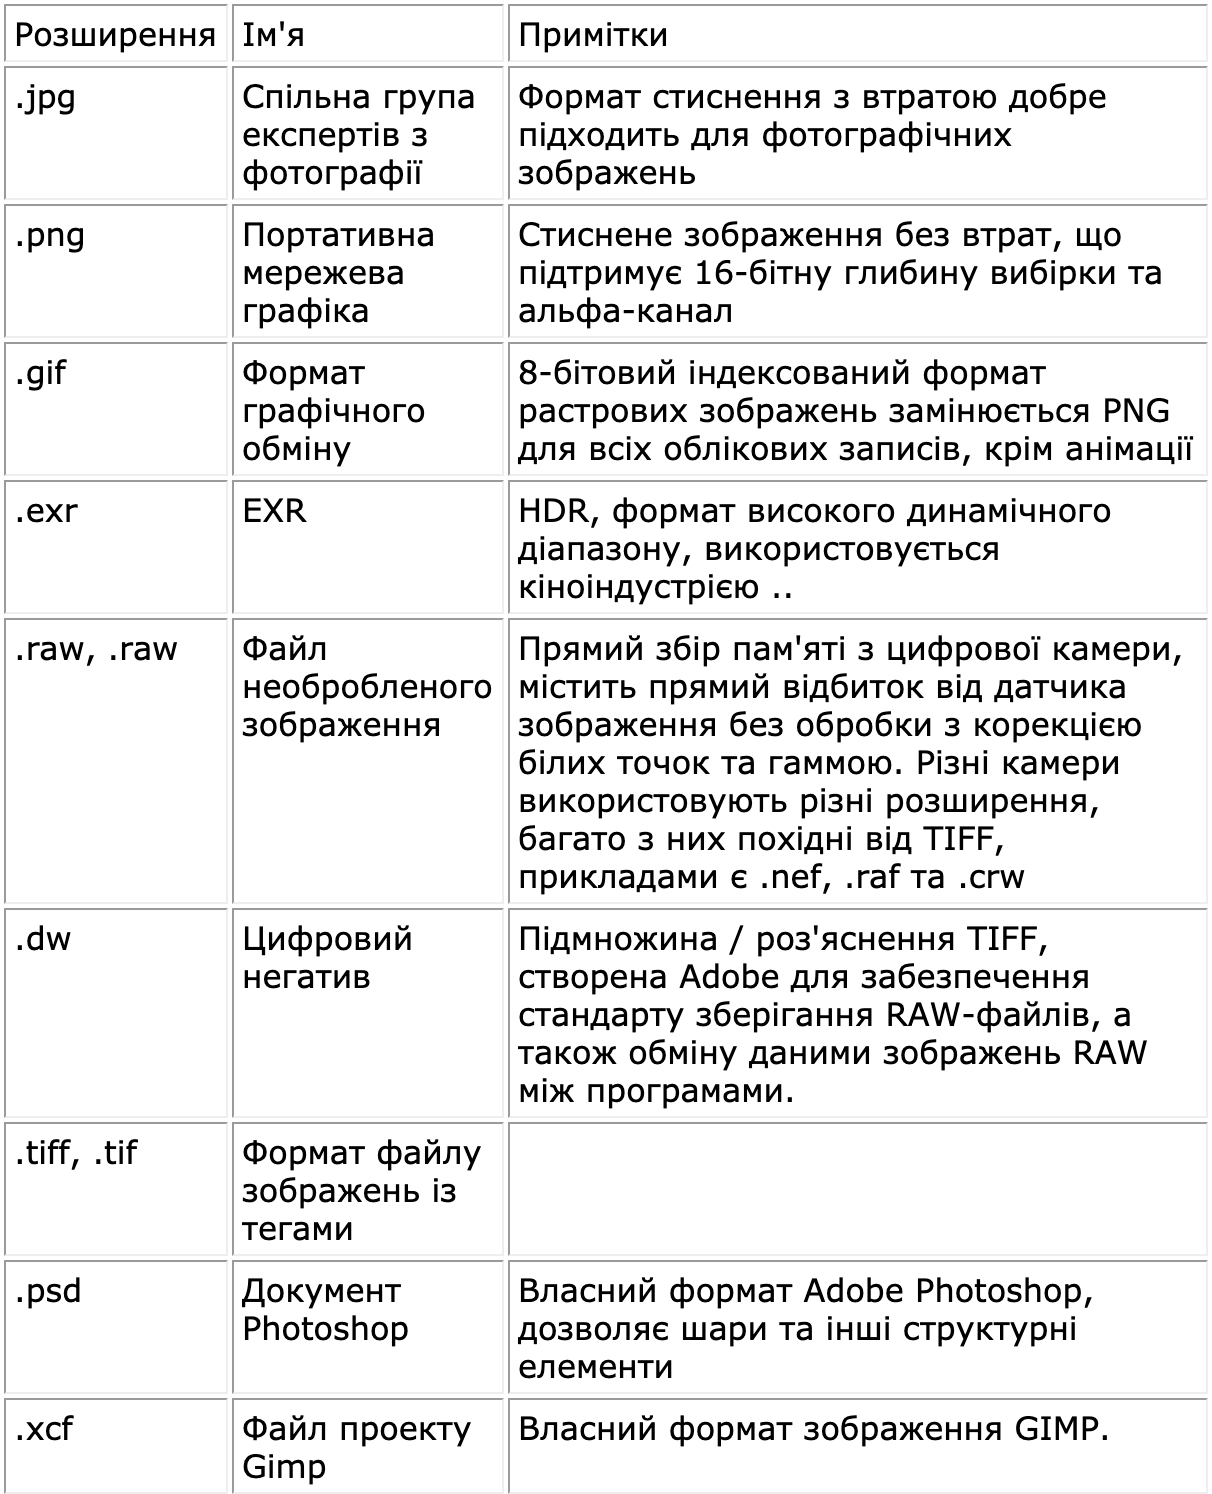
\includegraphics[scale=0.5]{image12.png}

        Рис. 12. Формати растрових файлів.
    \end{figure}

    \newpage

    \printbibliography[title={Список Літератури}]

\end{document}
